\chapter{Propuesta}\label{chapter:proposal}
 
    El objetivo de proponer el diseño de un sistema para generar resúmenes de eventos deportivos independiente de la fuente de datos 
planteó distintos retos. El primero de estos fue la necesidad de definir un esquema que permitiera abstraer las características 
generales del conjunto de deportes de enfrentamiento (enfrentamiento dos a dos). Junto con dicho esquema se necesitó 
definir una estructura común para la entrada de los datos que permitiera expresar los conocimientos del dominio. Se seleccionó 
una estructura basada en tuplas de cuatro elementos (cuatro-tuplas en lo adelante). A partir de esta estructura y en base 
al esquema de definición general se buscó poder determinar esquemas específicos para cada deporte que se fuera a incluir en el 
sistema. Cada uno de estos esquemas específicos son los que se encargan de definir un deporte de forma individual dentro del sistema.
Luego se realiza una propuesta general de diseño para concebir los modelos generadores de un deporte.
    
    En segunda instancia, se construye, en base a la propuesta, un esquema y su modelo correspondiente para generar 
resúmenes de partidos de fútbol. Lo mismo se realizó con un deporte de naturaleza diferente como el boxeo.

\section{Propuesta de Esquema General}

    Los deportes se pueden clasificar en la categoría de individuales o colectivos. En los deportes colectivos, las representaciones 
del enfrentamiento ocurren en base a equipos que agrupan a individuos. A su vez, en los deportes individuales son dos los contendientes.
Esta es la primera diferencia que se extrae en el análisis del conjunto de deportes. Las modalidades analizadas están representadas en \ref{tab:table_deportes_seleccionados}, 
clasificadas en individuales o colectivas.

% Please add the following required packages to your document preamble:
% \usepackage{multirow}
\begin{table}[]
    \begin{center}
    \begin{tabular}{|c|c|}
    \hline
    Colectivos                                                                                                                                          & Individuales                                                                                                     \\ \hline
    \multirow{5}{*}{\begin{tabular}[c]{@{}c@{}}Béisbol, Voleibol, \\ Fútbol, Tenis Dobles, \\ Baloncesto, Waterpolo, \\ Balonmano, Hockey\end{tabular}} & \multirow{5}{*}{\begin{tabular}[c]{@{}c@{}}Tenis, Esgrima, \\ Boxeo, Judo,\\ Lucha libre, Taekwondo\end{tabular}} \\
                                                                                                                                                        &                                                                                                                  \\
                                                                                                                                                        &                                                                                                                  \\
                                                                                                                                                        &                                                                                                                  \\
                                                                                                                                                        &                                                                                                                  \\ \hline
    \end{tabular}
    \caption{Deportes analizados}
    \label{tab:table_deportes_seleccionados}
    \end{center}
\end{table}

    De cada uno de estos deportes se analizó:

    \begin{itemize}
        \item Naturaleza de decisión: La mayoría de los deportes se definen como juegos 
        adversariales por acumulación de puntos. La entidad con mayor puntuación gana. Otros, como el tenis y el voleibol 
        se definen por cantidad de etapas ganadas (sets), y cada etapa se gana por puntos. A su vez, en el boxeo la definición 
        se deriva de votaciones de árbitros.
        \item Posibilidad de empate: Hay deportes como el fútbol en el que, según la competición o la fase de ésta, existe la posibilidad de 
        definirse sin ganadores ni perdedores.
        \item División de los eventos: La mayoría de los eventos se divide por etapas de tiempo.
        constante. Una excepción es el judo que ocurre de forma continua durante cuatro minutos. 
        \item Alargues de tiempo: La mayoría de los deportes, en caso de no definición en su tiempo reglamentario, presentan 
        etapas adicionales en forma punto de oro (ej. judo),  tiempos extras (ej. béisbol, fútbol), tiebreak (desempate, ej. voleibol, tenis).
        \item Roles: Dentro de los deportes los participantes ejercen roles, como puede ser su posición en los deportes colectivos. En los deportes 
        individuales estos roles no son tan explícitos.
        \item  Acciones principales: La definición de los eventos son las acciones relevantes que ocurren durante el tiempo de juego.
    \end{itemize}

    Del análisis también se extrajeron un conjunto de características que son comunes a los enfrentamientos deportivos: la sede, 
el público, la fecha. Asimismo, los enfrentamientos normalmente se encuadran dentro de un torneo, y existen distinciones entre categorías lo mismo sea 
de edad, sexo, u de otro tipo (ej. peso).

    A partir del análisis se definió un meta esquema general de tipos de entradas basado en una estructura de 
cuatro-tuplas de conocimiento.

\begin{table}[]
    \begin{center}

\begin{tabular}{|c|c|}
    \hline
    Tipo de Entrada  & Estructura                                                                                                               \\ \hline
    SEDE             & \begin{tabular}[c]{@{}c@{}}(TipoSEDE, \\ Nombre\\ Asistencia\\ Capacidad)\end{tabular}                                   \\ \hline
    TORNEO           & \begin{tabular}[c]{@{}c@{}}(TipoTORNEO\\  Nombre\\ Expresión de Género\\  Expresión de Categoría)\end{tabular}           \\ \hline
    ENFRENTAMIENTO   & \begin{tabular}[c]{@{}c@{}}(TipoENFRENTAMIENTO\\ Entidad\_1\\  Entidad\_2\\  Expresión de Fecha)\end{tabular}            \\ \hline
    ROLENJUEGO       & \begin{tabular}[c]{@{}c@{}}(TipoROLENJUEGO\\  Entidad del Rol\\  Entidad Complementaria\\ Rol Complementario)\end{tabular}   \\ \hline
    RESULTADOPARCIAL & \begin{tabular}[c]{@{}c@{}}(TipoRESULTADOPARCIAL\\ Entidad\\ Indicador de parcial\\ Expresión de puntuación)\end{tabular}    \\ \hline
    RESULTADOFINAL   & \begin{tabular}[c]{@{}c@{}}(TipoRESULTADOFINAL\\ Entidad\\ Expresión de puntuación\\  Descriptor de resultado)\end{tabular}  \\ \hline
    EVENTO           & \begin{tabular}[c]{@{}c@{}}(TipoEVENTO\\  Expresión de Tiempo\\ Entidad Protagonista\\  Entidad Complementaria)\end{tabular} \\ \hline
    \end{tabular}
        
    \end{center}
    \caption{Meta esquema general para definir las entradas de cada deporte}
    \label{tab:esquema_general}
\end{table}

    Cada cuatro-tupla tiene en la primera posición el tipo de entrada. El resto de los valores constituyen la base de información. Con cada tipo de entrada 
se encapsula un subconjunto de la información que se muestra, común al conjunto de deportes estudiados. 
    \\

%\pagebreak

    \textbf{Ejemplos abstractos de formación de entradas}\\

    Se presenta una meta representación de entradas basadas en el esquema general y su interpretación en el contexto del sistema.

    \begin{itemize}
        \item (SEDE, A, 1450, 1700) : El enfrentamiento ocurre en la sede de nombre A, con capacidad para 1700 espectadores, asistieron 1450.
        \item (TORNEO, B, F, categoría\_1) : El enfrentamiento pertenece al torneo B, femenino, en la categoría categoría\_1.
        \item (ENFRENTAMIENTO, contrincante\_A, contrincante\_B, 11-11-2022) : Se enfrentan contrincante\_A y contrincante\_B el 11 de noviembre de 2022. 
        \item (ROLENJUEGO, individuo\_A, entidad\_A, segundo\_rol) : El individuo\_A desarrolla primer\_rol y segundo\_rol respecto a entidad\_A.
        \item RESULTADOPARCIAL:
            \begin{itemize}
                \item (RESULTADOPARCIAL, contrincante\_A , P, X): En el parcial P, contrincante\_A tiene X puntos.
                \item (RESULTADOPARCIAL, contrincante\_B , P, Y): En el parcial P, contrincante\_B tiene Y puntos.
            \end{itemize}
        \item RESULTADOFINAL:
            \begin{itemize}
                \item (RESULTADOFINAL, contrincante\_A, X, Derrota): El contrincante\_A perdió con X puntos.
                \item (RESULTADOFINAL, contrincante\_B, Y, Victoria): El contrincante\_B ganó con Y puntos.
            \end{itemize}
        \item EVENTO: 
            \begin{itemize}
                \item (EVENTO, tiempo\_x , individuo\_A, “”): En el tiempo\_x, el individuo\_A protagonizó el EVENTO
                \item (EVENTO, tiempo\_y, individuo\_A, individuo\_B): En el tiempo\_y, individuo\_A protagonizó el EVENTO en 
                complemento de (en oposición de, en beneficio de, en perjuicio de, en relación con, respecto a) individuo\_B. 
            \end{itemize}
    \end{itemize}

   A partir del meta esquema general es posible definir el diseño de los esquemas específicos de cada deporte, con sus tipos particulares para cada entrada y su forma de interpretar 
cada uno de los valores. Los esquemas de cada deporte tienen que ser capaces de expresar la información del mismo y, a través de ella, 
generar textos que describan el enfrentamiento. 

%A continuación se presenta la definición para dos deportes de naturaleza y estructura muy dispar: el fútbol y 
%el boxeo.

\section{Metodología para la conformación de los esquemas específicos}

    Primero, es necesario tener en cuenta que el meta esquema planteado anteriormente busca la abstracción de conceptos comunes. Estos 
conceptos necesitan, al menos los referentes a los roles, eventos y resultados, ser llevados a su expresión específica dentro de una modalidad 
deportiva. A su vez, se deben diferenciar los conceptos de: capacidad de representación y obligación de representación. Que el esquema permita definir 
un tipo de información determinada no significa que todos los deportes expresen necesariamente ese concepto. Además, es posible que se conciban distintos 
esquemas específicos para un mismo deporte. Esto depende de cómo cada modelo sea representado.

    La representación de un deporte en un esquema específico a partir del esquema general propuesto necesita del análisis de sus características. 
Se debe realizar un estudio que permita detallar las situaciones que presenta el deporte y representarlas basado en eventos. A partir de 
estudiar las reglamentaciones se separa al deporte en cuanto a su categoría: individual o colectivo. 

    Para los deportes colectivos la expresión de los roles de los deportistas se encuentra mínimamente definida a partir del concepto de 
alineación. Esta serie de deportes tienen un conjunto de individuos que inician las disputas de los encuentros y otros que ingresan a raíz de decisiones 
que se toman durante el transcurso de los mismos. Además, se pueden expresar conceptos como las disposiciones que ocupa cada deportista dentro del equipo. En este 
tipo de información, la \textit{entidad complementaria} que define la tupla de \textit{ROLENJUEGO} sería el equipo del deportista.
    En el caso de los deportes individuales, los roles no se expresan tan claramente. Aun así, es posible identificar roles de representación, ya sea de un 
país, una delegación, un equipo multi categoría. Un ejemplo fuera de los deportes de enfrentamiento se encuentra en la fórmula 1, donde los competidores 
representan a escuderías durante las carreras.

    En lo referido a los parciales, se necesita determinar las etapas en las que trascurre un enfrentamiento en caso de que este ocurra por etapas. La información 
de los parciales permite al sistema desambiguar situaciones que ocurren durante los enfrentamientos, así como da la posibilidad de dotar de más información 
la narrativa. Para conformar las tuplas de \textit{RESULTADOPARCIAL}, es necesario determinar si existe uno o m\'as tipos de segmentación dentro del enfrentamiento, así como 
lograr una expresión identificativa que sea única para cada una.

    La expresión de los eventos es la que dota principalmente de capacidad descriptiva a los modelos. Los eventos, acciones que se suceden en un deporte, son la esencia de 
este y por esa razón son la información fundamental que sobre ellos se transmite, más allá del resultado. Para expresar los eventos es necesario en primera instancia determinar cuáles 
son los que existen dentro de la modalidad seleccionada. A partir de esto, definir si para su expresión es necesario el concepto de antagonista como sujeto no protagonista en la acción.
También se debe determinar una expresión temporal que identifique de forma única y cronológica la secuencia de eventos. De esta forma no se generan ambigüedades a la hora de que los 
modelos interpreten los mismos.

    Los datos referentes a la sede, el público, el torneo, el resultado y las categorías se expresan de forma más directa. Queda en decisión del realizador del esquema y su modelo específico 
determinar qué informaciones constituyen un requerimiento en el contexto de la generación del resumen y cuáles son complementos informativos. Es decir, el modelo sería capaz de lidiar con 
la ausencia de determinados datos. 


\section{Propuesta de diseño para los modelos generadores}

    A partir de la definición de un esquema para la conformación de las tuplas de conocimiento de un deporte determinado se debe concebir 
un modelo que transforme esa entrada en un resumen textual. En la sección se propone un enfoque adaptable para los modelos de generación siguiendo 
los requerimientos de los sistemas de GLN y las propuestas presentes en la literatura para idiomas distintos al español.

    Como paso previo necesario para la conversión de los datos en resúmenes textuales se define qué información es relevante a 
incluir en la salida y bajo qué estructura. Como los enfrentamientos deportivos son eventos repetitivos, cuyo conocimiento está bien 
definido, el enfoque basado en corpus es adaptable para la planificación del contenido. Reiter y Dale \brackcite{reiter_dale_2000} plantearon que tras 
el análisis de un conjunto de textos que aborden el dominio es posible determinar la estructura subyacente, así como la información relevante a incluir. 
En los reportes deportivos es posible identificar una estructura con una presentación, donde se incluye el resultado e información general, 
seguido de una mención de los eventos de mayor importancia. 


\begin{figure}[!]
    \begin{center}
        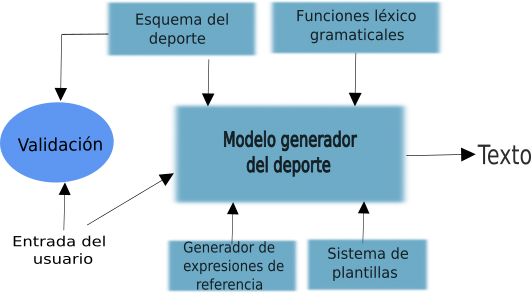
\includegraphics[scale=0.9]{Graphics/arquitecturatesisOKFINAL.png}
    \end{center}
    \caption{Arquitectura de modelo propuesta}
    \label{arquitecturadelmodeloOK}
\end{figure}

    La arquitectura general planteada se presenta en \ref{arquitecturadelmodeloOK} y constituye una 
adaptación de la propuesta de Aires \brackcite{aires2016automatic} que a su vez sigue un enfoque basado en la propuesta de Theune y col. \brackcite{theune2001data}. 
A diferencia de las mismas, el sistema propuesto no consume bases de conocimiento específicas, ya que busca adaptarse al hecho general del deporte a
abordar. Un sistema sencillo para generar expresiones de referencia se incluye con el objetivo de que los modelos generen un texto más fluido.

    Como se analizó en el capítulo anterior (\ref{chapter:state-of-the-art}), las tareas de los sistemas de generación de texto a partir de datos se pueden dividir en 
dos etapas: la referente al contenido a representar y su estructura (planificación del contenido) y la de realización lingüística. La planificación del contenido 
viene dada por la estructura extraída de los textos analizados. Para la etapa de realización, se propone un sistema basado en reglas y plantillas.

    \subsubsection{Realización lingüística}
 
    En la etapa de realización del texto se ven unificadas las tareas de carácter lingüístico tal y como se presentó en \ref{chapter:state-of-the-art}. 
En este proceso se determinan las palabras y expresiones con las que exponer el contenido seleccionado bajo la estructura definida. El enfoque basado en reglas 
y llenado de plantilla es de los más utilizados por el control que otorga sobre la producción del texto (\ref{subsection:lexicalizacion}). Tiene la ventaja de que 
se asegura la calidad estructural del texto producido, así como permite dotar de variabilidad a las salidas tal y como se discutió en el capítulo 
anterior (\ref{subsection:realizcion}).

    Las plantillas se utilizan dentro del modelo para conformar estructuras más complejas en forma de oraciones. Cada conjunto 
de plantillas dentro del sistema pertenece a una parte de la estructura del texto. Para cada contexto se conciben varias plantillas que brindan opciones para expresar la información relativa a una idea.

    Las plantillas pueden o no presentar ranuras para completar con información. Las ranuras se utilizan de la forma: \textit{$<$ dato $>$} donde 
\textit{dato} se sustituye por el valor de la variable que representa. Para dotar de facilidad al sistema a la hora de adaptarse a eventos de 
ambos géneros, se puede utilizar dentro de las plantillas expresiones como \textit{\$ expresión dependiente del género \$}, donde \textit{“expresión dependiente del género” }
se sustituye por su expresión de género correcta dentro del contexto a través de una de las funciones léxicas. El caracter “@” también se utiliza dentro de las plantillas 
para hacer distinciones de género. Por ejemplo en la frase: \textit{amb@s se golpearon}, el “@” se sustituye por “a” o por “o” en dependencia del género.
\\

\textbf{Funciones lingüísticas}\\

    Las funciones lingüísticas tienen el objetivo de mejorar la calidad del texto producido. Asimismo, buscan asegurar su correcta estructura gramatical. Una vez constituida una oración a partir de unificar plantillas de expresiones, una función se encarga de dotar de un 
formato a la misma. Se colocan las mayúsculas correspondientes al inicio, así como los puntos finales. Otra función se emplea para eliminar errores gramaticales o de 
estructura que se presentan durante la unión de las plantillas. Se eliminan los espacios en blanco múltiples, se corrigen los signos de puntuación así como los artículos 
repetidos y las construcciones mal formadas, como por ejemplo “de el”.

Otras funciones léxicas se utilizan para dar mayor fluidez al texto, como las que transforman expresiones numéricas en texto, por ejemplo, “3” por “tres”.
\\

\textbf{Generador de expresiones de referencia}\\

Las expresiones de referencia son las que permiten identificar unívocamente a una entidad dentro de un contexto \brackcite{reiter_dale_2000,Gatt2018SurveyOT}. 
Un sistema de expresiones de referencia debe determinar si la entidad a referenciar ha sido mencionada previamente, ya que existe una diferenciación entre la 
introducción de una entidad y su referencia tardía, tal y como se trató en el capítulo anterior (\ref{subsection:expreferencia}). A su vez, la expresión seleccionada 
para referirse a una entidad debe tener en cuenta el resto de entidades del dominio. Por ejemplo, en un evento donde “Alejandro González” y “Pedro González” sean 
protagonistas, la expresión “González” resulta ambigua. Se propone un generador de expresiones de referencia basado en los nombres propios de los integrantes del 
enfrentamiento, utilizando los apellidos como referencias tardías y el nombre completo en la introducción.



    


